% Options for packages loaded elsewhere
\PassOptionsToPackage{unicode}{hyperref}
\PassOptionsToPackage{hyphens}{url}
%
\documentclass[
  ignorenonframetext,
]{beamer}
\usepackage{pgfpages}
\setbeamertemplate{caption}[numbered]
\setbeamertemplate{caption label separator}{: }
\setbeamercolor{caption name}{fg=normal text.fg}
\beamertemplatenavigationsymbolsempty
% Prevent slide breaks in the middle of a paragraph
\widowpenalties 1 10000
\raggedbottom
\setbeamertemplate{part page}{
  \centering
  \begin{beamercolorbox}[sep=16pt,center]{part title}
    \usebeamerfont{part title}\insertpart\par
  \end{beamercolorbox}
}
\setbeamertemplate{section page}{
  \centering
  \begin{beamercolorbox}[sep=12pt,center]{section title}
    \usebeamerfont{section title}\insertsection\par
  \end{beamercolorbox}
}
\setbeamertemplate{subsection page}{
  \centering
  \begin{beamercolorbox}[sep=8pt,center]{subsection title}
    \usebeamerfont{subsection title}\insertsubsection\par
  \end{beamercolorbox}
}
\AtBeginPart{
  \frame{\partpage}
}
\AtBeginSection{
  \ifbibliography
  \else
    \frame{\sectionpage}
  \fi
}
\AtBeginSubsection{
  \frame{\subsectionpage}
}

\usepackage{amsmath,amssymb}
\usepackage{iftex}
\ifPDFTeX
  \usepackage[T1]{fontenc}
  \usepackage[utf8]{inputenc}
  \usepackage{textcomp} % provide euro and other symbols
\else % if luatex or xetex
  \usepackage{unicode-math}
  \defaultfontfeatures{Scale=MatchLowercase}
  \defaultfontfeatures[\rmfamily]{Ligatures=TeX,Scale=1}
\fi
\usepackage{lmodern}
\ifPDFTeX\else  
    % xetex/luatex font selection
\fi
% Use upquote if available, for straight quotes in verbatim environments
\IfFileExists{upquote.sty}{\usepackage{upquote}}{}
\IfFileExists{microtype.sty}{% use microtype if available
  \usepackage[]{microtype}
  \UseMicrotypeSet[protrusion]{basicmath} % disable protrusion for tt fonts
}{}
\makeatletter
\@ifundefined{KOMAClassName}{% if non-KOMA class
  \IfFileExists{parskip.sty}{%
    \usepackage{parskip}
  }{% else
    \setlength{\parindent}{0pt}
    \setlength{\parskip}{6pt plus 2pt minus 1pt}}
}{% if KOMA class
  \KOMAoptions{parskip=half}}
\makeatother
\usepackage{xcolor}
\newif\ifbibliography
\setlength{\emergencystretch}{3em} % prevent overfull lines
\setcounter{secnumdepth}{-\maxdimen} % remove section numbering

\usepackage{color}
\usepackage{fancyvrb}
\newcommand{\VerbBar}{|}
\newcommand{\VERB}{\Verb[commandchars=\\\{\}]}
\DefineVerbatimEnvironment{Highlighting}{Verbatim}{commandchars=\\\{\}}
% Add ',fontsize=\small' for more characters per line
\usepackage{framed}
\definecolor{shadecolor}{RGB}{241,243,245}
\newenvironment{Shaded}{\begin{snugshade}}{\end{snugshade}}
\newcommand{\AlertTok}[1]{\textcolor[rgb]{0.68,0.00,0.00}{#1}}
\newcommand{\AnnotationTok}[1]{\textcolor[rgb]{0.37,0.37,0.37}{#1}}
\newcommand{\AttributeTok}[1]{\textcolor[rgb]{0.40,0.45,0.13}{#1}}
\newcommand{\BaseNTok}[1]{\textcolor[rgb]{0.68,0.00,0.00}{#1}}
\newcommand{\BuiltInTok}[1]{\textcolor[rgb]{0.00,0.23,0.31}{#1}}
\newcommand{\CharTok}[1]{\textcolor[rgb]{0.13,0.47,0.30}{#1}}
\newcommand{\CommentTok}[1]{\textcolor[rgb]{0.37,0.37,0.37}{#1}}
\newcommand{\CommentVarTok}[1]{\textcolor[rgb]{0.37,0.37,0.37}{\textit{#1}}}
\newcommand{\ConstantTok}[1]{\textcolor[rgb]{0.56,0.35,0.01}{#1}}
\newcommand{\ControlFlowTok}[1]{\textcolor[rgb]{0.00,0.23,0.31}{\textbf{#1}}}
\newcommand{\DataTypeTok}[1]{\textcolor[rgb]{0.68,0.00,0.00}{#1}}
\newcommand{\DecValTok}[1]{\textcolor[rgb]{0.68,0.00,0.00}{#1}}
\newcommand{\DocumentationTok}[1]{\textcolor[rgb]{0.37,0.37,0.37}{\textit{#1}}}
\newcommand{\ErrorTok}[1]{\textcolor[rgb]{0.68,0.00,0.00}{#1}}
\newcommand{\ExtensionTok}[1]{\textcolor[rgb]{0.00,0.23,0.31}{#1}}
\newcommand{\FloatTok}[1]{\textcolor[rgb]{0.68,0.00,0.00}{#1}}
\newcommand{\FunctionTok}[1]{\textcolor[rgb]{0.28,0.35,0.67}{#1}}
\newcommand{\ImportTok}[1]{\textcolor[rgb]{0.00,0.46,0.62}{#1}}
\newcommand{\InformationTok}[1]{\textcolor[rgb]{0.37,0.37,0.37}{#1}}
\newcommand{\KeywordTok}[1]{\textcolor[rgb]{0.00,0.23,0.31}{\textbf{#1}}}
\newcommand{\NormalTok}[1]{\textcolor[rgb]{0.00,0.23,0.31}{#1}}
\newcommand{\OperatorTok}[1]{\textcolor[rgb]{0.37,0.37,0.37}{#1}}
\newcommand{\OtherTok}[1]{\textcolor[rgb]{0.00,0.23,0.31}{#1}}
\newcommand{\PreprocessorTok}[1]{\textcolor[rgb]{0.68,0.00,0.00}{#1}}
\newcommand{\RegionMarkerTok}[1]{\textcolor[rgb]{0.00,0.23,0.31}{#1}}
\newcommand{\SpecialCharTok}[1]{\textcolor[rgb]{0.37,0.37,0.37}{#1}}
\newcommand{\SpecialStringTok}[1]{\textcolor[rgb]{0.13,0.47,0.30}{#1}}
\newcommand{\StringTok}[1]{\textcolor[rgb]{0.13,0.47,0.30}{#1}}
\newcommand{\VariableTok}[1]{\textcolor[rgb]{0.07,0.07,0.07}{#1}}
\newcommand{\VerbatimStringTok}[1]{\textcolor[rgb]{0.13,0.47,0.30}{#1}}
\newcommand{\WarningTok}[1]{\textcolor[rgb]{0.37,0.37,0.37}{\textit{#1}}}

\providecommand{\tightlist}{%
  \setlength{\itemsep}{0pt}\setlength{\parskip}{0pt}}\usepackage{longtable,booktabs,array}
\usepackage{calc} % for calculating minipage widths
\usepackage{caption}
% Make caption package work with longtable
\makeatletter
\def\fnum@table{\tablename~\thetable}
\makeatother
\usepackage{graphicx}
\makeatletter
\newsavebox\pandoc@box
\newcommand*\pandocbounded[1]{% scales image to fit in text height/width
  \sbox\pandoc@box{#1}%
  \Gscale@div\@tempa{\textheight}{\dimexpr\ht\pandoc@box+\dp\pandoc@box\relax}%
  \Gscale@div\@tempb{\linewidth}{\wd\pandoc@box}%
  \ifdim\@tempb\p@<\@tempa\p@\let\@tempa\@tempb\fi% select the smaller of both
  \ifdim\@tempa\p@<\p@\scalebox{\@tempa}{\usebox\pandoc@box}%
  \else\usebox{\pandoc@box}%
  \fi%
}
% Set default figure placement to htbp
\def\fps@figure{htbp}
\makeatother

% Add this to your preamble
\usepackage{xcolor}
\setbeamercolor{block title example}{fg=black, bg=olive!30}
\setbeamercolor{block body example}{fg=black, bg=olive!10}

% \usepackage{etoolbox}
%
% % Make top-level itemize lists incremental, but keep nested lists static
% \makeatletter
% \renewenvironment{itemize}
%   {\only<+->{\begin{list}{$\bullet$}{\leftmargin=1.5em}}} % Top-level incremental
%   {\end{list}}
% \makeatother
\makeatletter
\@ifpackageloaded{caption}{}{\usepackage{caption}}
\AtBeginDocument{%
\ifdefined\contentsname
  \renewcommand*\contentsname{Table of contents}
\else
  \newcommand\contentsname{Table of contents}
\fi
\ifdefined\listfigurename
  \renewcommand*\listfigurename{List of Figures}
\else
  \newcommand\listfigurename{List of Figures}
\fi
\ifdefined\listtablename
  \renewcommand*\listtablename{List of Tables}
\else
  \newcommand\listtablename{List of Tables}
\fi
\ifdefined\figurename
  \renewcommand*\figurename{Figure}
\else
  \newcommand\figurename{Figure}
\fi
\ifdefined\tablename
  \renewcommand*\tablename{Table}
\else
  \newcommand\tablename{Table}
\fi
}
\@ifpackageloaded{float}{}{\usepackage{float}}
\floatstyle{ruled}
\@ifundefined{c@chapter}{\newfloat{codelisting}{h}{lop}}{\newfloat{codelisting}{h}{lop}[chapter]}
\floatname{codelisting}{Listing}
\newcommand*\listoflistings{\listof{codelisting}{List of Listings}}
\makeatother
\makeatletter
\makeatother
\makeatletter
\@ifpackageloaded{caption}{}{\usepackage{caption}}
\@ifpackageloaded{subcaption}{}{\usepackage{subcaption}}
\makeatother
\makeatletter
\@ifpackageloaded{tikz}{}{\usepackage{tikz}}
\makeatother
        \newcommand*\circled[1]{\tikz[baseline=(char.base)]{
          \node[shape=circle,draw,inner sep=1pt] (char) {{\scriptsize#1}};}}  
                  

\usepackage{bookmark}

\IfFileExists{xurl.sty}{\usepackage{xurl}}{} % add URL line breaks if available
\urlstyle{same} % disable monospaced font for URLs
\hypersetup{
  pdftitle={ORCA},
  pdfauthor={Ankush Jain},
  hidelinks,
  pdfcreator={LaTeX via pandoc}}


\title{ORCA}
\author{Ankush Jain}
\date{}

\begin{document}
\frame{\titlepage}


\begin{frame}{Agenda -- 20250304}
\phantomsection\label{agenda-20250304}
\begin{itemize}
\tightlist
\item
  Github Projects
\item
  Dashboard
\item
  Ideas on comparing with tracing

  \begin{itemize}
  \tightlist
  \item
    Visualization
  \item
    Performance
  \end{itemize}
\item
  Sheng wrote a benchmark
\item
  Timestep-linked Two-Phase Commit (TS2PC)
\end{itemize}
\end{frame}

\begin{frame}[fragile]{Timestep-linked Two-Phase Commit (TS2PC)}
\phantomsection\label{timestep-linked-two-phase-commit-ts2pc}
\begin{itemize}
\tightlist
\item
  Motivation: negligible-cost control semantics at scale

  \begin{itemize}
  \tightlist
  \item
    Fundamental interface between BSP/async worlds
  \end{itemize}
\end{itemize}

\pause

\begin{itemize}
\tightlist
\item
  Control messages accumulate at ranks async, applied at \texttt{ts+X}

  \begin{itemize}
  \tightlist
  \item
    \texttt{X} here is a speculative delta: a function of \emph{latency}
  \item
    Can be learned online. If a 2PC round fails, \texttt{X++}
  \end{itemize}
\end{itemize}

\pause

\begin{itemize}
\tightlist
\item
  Advantage: allows arbitrary QoS mechanisms

  \begin{itemize}
  \tightlist
  \item
    ORCA: can not setup your QoS for you
  \item
    But can tolerate arbitrary delays
  \end{itemize}
\end{itemize}

\pause

\begin{itemize}
\tightlist
\item
  Essentially solves the control path for all steering usecases

  \begin{itemize}
  \tightlist
  \item
    Control message broadcast using an on-fabric overlay
  \item
    Responses coalesced using the same overlay
  \item
    Consistent and opcode-independent
  \end{itemize}
\end{itemize}
\end{frame}

\begin{frame}{TS2PC Figure}
\phantomsection\label{ts2pc-figure}
\begin{figure}[H]

{\centering \pandocbounded{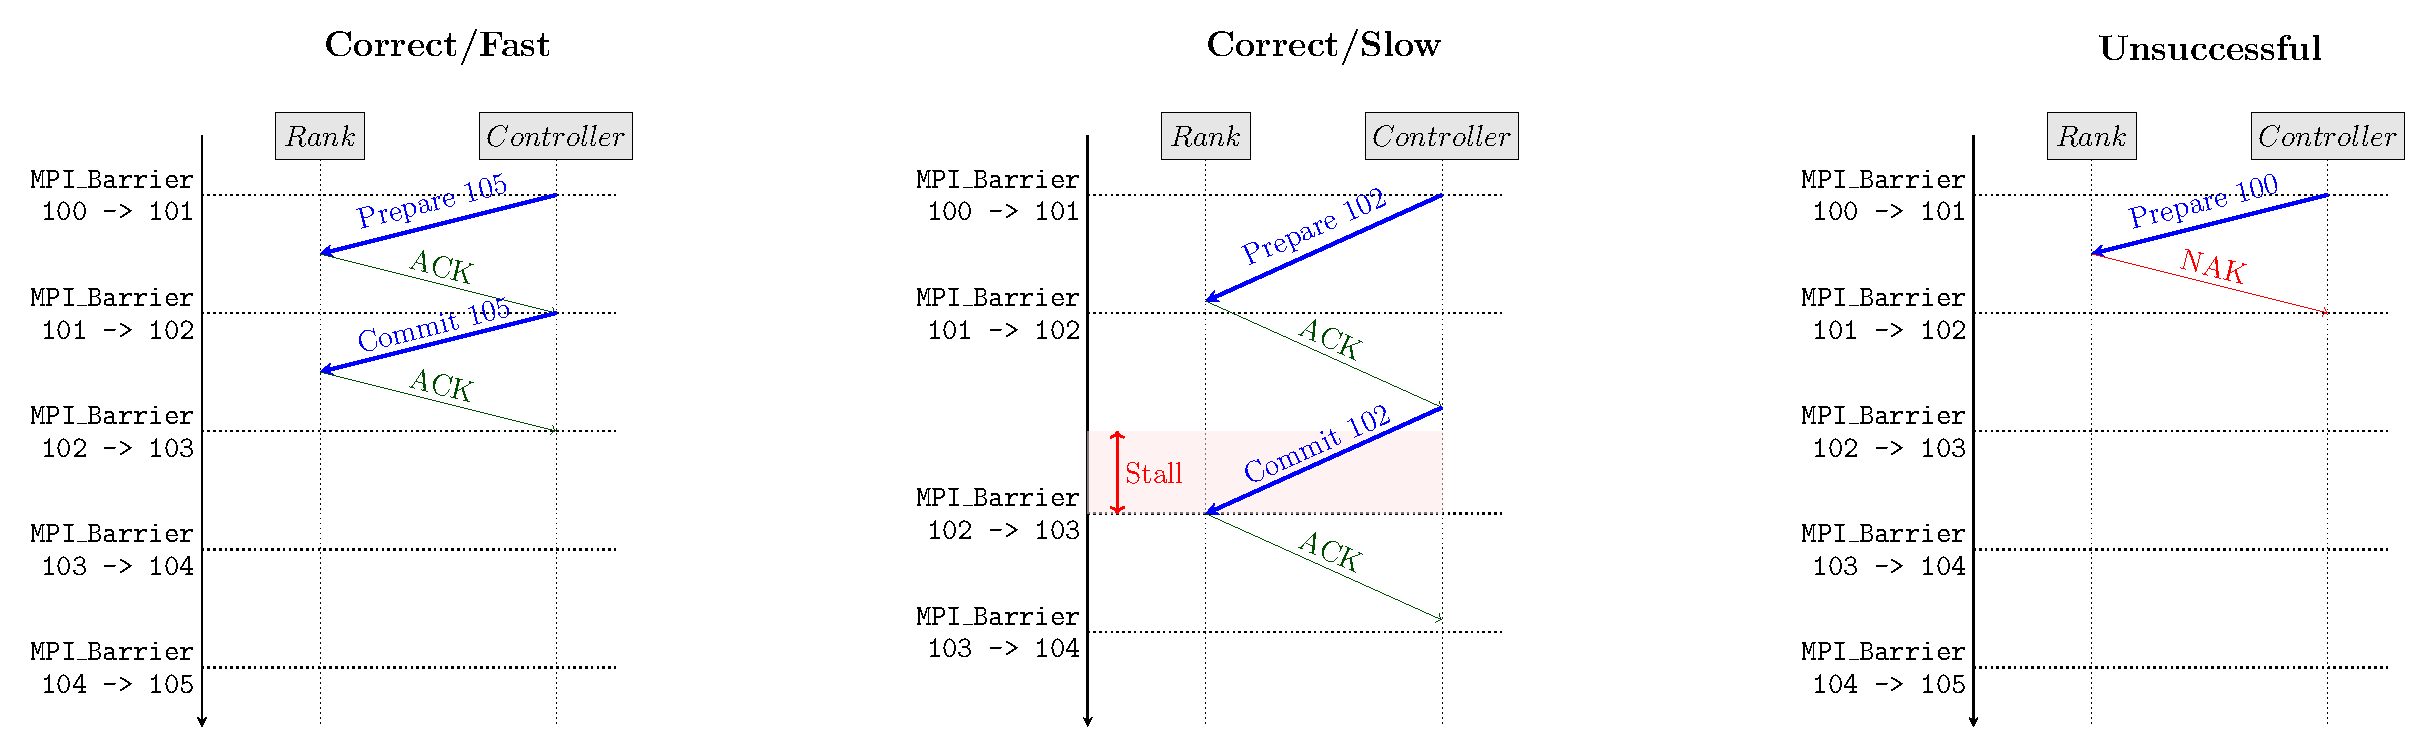
\includegraphics[keepaspectratio]{../tikz-exps/pdf/ts2pc.pdf}}

}

\caption{TS2PC}

\end{figure}%
\end{frame}

\begin{frame}[fragile]{TS2PC Protocol}
\phantomsection\label{ts2pc-protocol}
\phantomsection\label{annotated-cell-1}%
\begin{Shaded}
\begin{Highlighting}[]
\NormalTok{\{}
\NormalTok{   txnseq: int \# \textless{}1\textgreater{}}
\NormalTok{   txnts: int \# \textless{}2\textgreater{}}
\NormalTok{   phase: PREPARE | COMMIT | ABORT}
\NormalTok{   cmd: union \{}
\NormalTok{     op: enum}
\NormalTok{     args: struct}
\NormalTok{   \}}
\NormalTok{\}}
\end{Highlighting}
\end{Shaded}

\begin{description}
\tightlist
\item[\circled{1}]
\texttt{txnseq}: unique transaction identifier
\item[\circled{2}]
\texttt{txnts}: timestamp at which to apply txn
\end{description}
\end{frame}

\begin{frame}[fragile]{TS2PC Response}
\phantomsection\label{ts2pc-response}
\phantomsection\label{annotated-cell-2}%
\begin{Shaded}
\begin{Highlighting}[]
\NormalTok{\{}
\NormalTok{  txnseq: int}
\NormalTok{  response: PREPARE\_ACK | PREPARE\_NACK }
\NormalTok{            | COMMIT\_ACK | ABORT\_ACK \# \textless{}1\textgreater{}}
\NormalTok{  rank\_range: [begin, end) \# \textless{}2\textgreater{}}
\NormalTok{\}}
\end{Highlighting}
\end{Shaded}

\begin{description}
\tightlist
\item[\circled{1}]
COMMIT\_NACK and ABORT\_NACK undefined
\item[\circled{2}]
\texttt{rank\_range}: range of ranks this response represents
\end{description}
\end{frame}

\begin{frame}[fragile]{TS2PC: Some Code-level Details}
\phantomsection\label{ts2pc-some-code-level-details}
\begin{itemize}
\tightlist
\item
  Responses can be coalesced by the overlay using reducers

  \begin{itemize}
  \tightlist
  \item
    (Reducers implemented, coalescing TODO)
  \end{itemize}
\end{itemize}

\pause

\begin{itemize}
\tightlist
\item
  Core 2PC module has server and client

  \begin{itemize}
  \tightlist
  \item
    Agnostic to overlay/XDR etc.
  \item
    Server just issues \texttt{txnseq}s and tracks state
  \item
    Client implemented within MPI-side hooks \texttt{PretimestepAdvance}
    and \texttt{PosttimestepAdvance}
  \end{itemize}
\end{itemize}

\pause

\begin{itemize}
\tightlist
\item
  Controller will have two 2PC \emph{domains}

  \begin{itemize}
  \tightlist
  \item
    MPI and AGGs form separate domains
  \item
    MPI: 2PC used for toggling probes, tuning etc.
  \item
    AGGs: 2PC used to install new queries etc.
  \end{itemize}
\end{itemize}
\end{frame}

\begin{frame}[fragile]{TS2PC: Some More Details}
\phantomsection\label{ts2pc-some-more-details}
\begin{itemize}
\tightlist
\item
  Designed to block on \texttt{TimestepAdvance} at MPI if txns for
  \texttt{ts+1} \texttt{PREPARE}d but not \texttt{COMMIT}ed or
  \texttt{ABORT}ed
\end{itemize}

\pause

\begin{itemize}
\tightlist
\item
  Catch 1: servicing message queues should not block

  \begin{itemize}
  \tightlist
  \item
    (Messages needed to unblock may be stuck in a queue)
  \item
    We have been trying to keep the MPI thread count small
  \end{itemize}
\end{itemize}

\pause

\begin{itemize}
\tightlist
\item
  Catch 2: think of \texttt{PAUSE} and \texttt{RESUME} control messages

  \begin{itemize}
  \tightlist
  \item
    Most control messages are for a future timestep (\texttt{ts+2})
  \item
    A \texttt{PAUSE}d simulation will never get to \texttt{ts+2} to
    process \texttt{RESUME}
  \end{itemize}
\end{itemize}

\pause

\begin{itemize}
\tightlist
\item
  Solution: another state machine

  \begin{itemize}
  \tightlist
  \item
    \texttt{MPI\_BREAK}: keep looping in the hook, do not return control
  \item
    \texttt{MPI\_BREAKSYNC}: keep looping but apply all CMDs immediately

    \begin{itemize}
    \tightlist
    \item
      Bypass the TS2PC layer
    \end{itemize}
  \item
    \texttt{MPI\_RESUME}: return control to the simulation
  \end{itemize}
\end{itemize}
\end{frame}

\begin{frame}[fragile]{TS2PC: Status}
\phantomsection\label{ts2pc-status}
\begin{itemize}
\tightlist
\item
  Core 2PC module: done
\item
  2PC for MPI domain: done
\item
  Response coalescing: TODO

  \begin{itemize}
  \tightlist
  \item
    Currently all ranks respond directly to CTL
  \end{itemize}
\item
  2PC for AGG domain: TODO
\item
  Opcode implementation: TODO
\item
  \texttt{BREAK} states: TODO
\end{itemize}
\end{frame}

\begin{frame}[fragile]{The Tracing Story}
\phantomsection\label{the-tracing-story}
\begin{itemize}
\tightlist
\item
  Original problem: how to implement a streaming tracing view

  \begin{itemize}
  \tightlist
  \item
    Implement custom streaming trace visualization?
  \item
    Rendered element volume grows monotonically
  \item
    Way beyond our scope
  \end{itemize}
\end{itemize}

\pause

\begin{itemize}
\tightlist
\item
  Solution: tracing is not a common-case view

  \begin{itemize}
  \tightlist
  \item
    We collect telemetry in nicely partitioned Arrow on-disk
  \item
    Export slices as traces

    \begin{itemize}
    \tightlist
    \item
      \texttt{export-trace\ timesteps\ 200-1000\ ranks\ 512-1024}
    \end{itemize}
  \item
    Generates OTF2 or TraceEvent files
  \item
    Realtime view is aggregates of telemetry
  \item
    (This is not an ORCA problem, this is a viz tooling problem)
  \end{itemize}
\end{itemize}

\pause

\begin{itemize}
\tightlist
\item
  This also allows comparing with OTF2 as an index

  \begin{itemize}
  \tightlist
  \item
    OTF2: MPI telemetry standard
  \item
    Bulky file format, not indexed for analyses
  \item
    ORCA telemetry is timestep-partitioned
  \item
    Compare range query performance
  \end{itemize}
\end{itemize}

\pause

\begin{itemize}
\tightlist
\item
  Other export option: Perfetto/TraceEvent
\end{itemize}
\end{frame}

\begin{frame}{Next Steps}
\phantomsection\label{next-steps}
\begin{itemize}
\tightlist
\item
  Finish basic 2PC
\item
  Test and validate single-aggregator ORCA with benchmarks
\item
  Dashboard etc.
\item
  Trace export tools
\item
  After: distributed datafusion
\end{itemize}
\end{frame}




\end{document}
